%********************************************************************************************
%
% Filename : 01_Introduction.tex
%
% Function : Introduction
%
% Author : XingzhongLi
%
% Date : 2018/11
%
%********************************************************************************************

In the field of geophysics, especially in seismology, we usually want to get a grid model 
to do our calculation on it. But there is no ready-made grid model, we have to generate 
the grid model from other models. For example, there are many layered models in nature. 
So how to generate a grid model from a layered model is our problem. \par

As shown in Figure \ref{fig:Layered_model}, a typical layered model, with two undulating 
interfaces. And each layer has a P wave velocity : 4.0 km/s in the first layer, 5.0 km/s 
in the second layer and 6.0 km/s in the third layer.
\begin{figure}[h]
    \begin{center}
        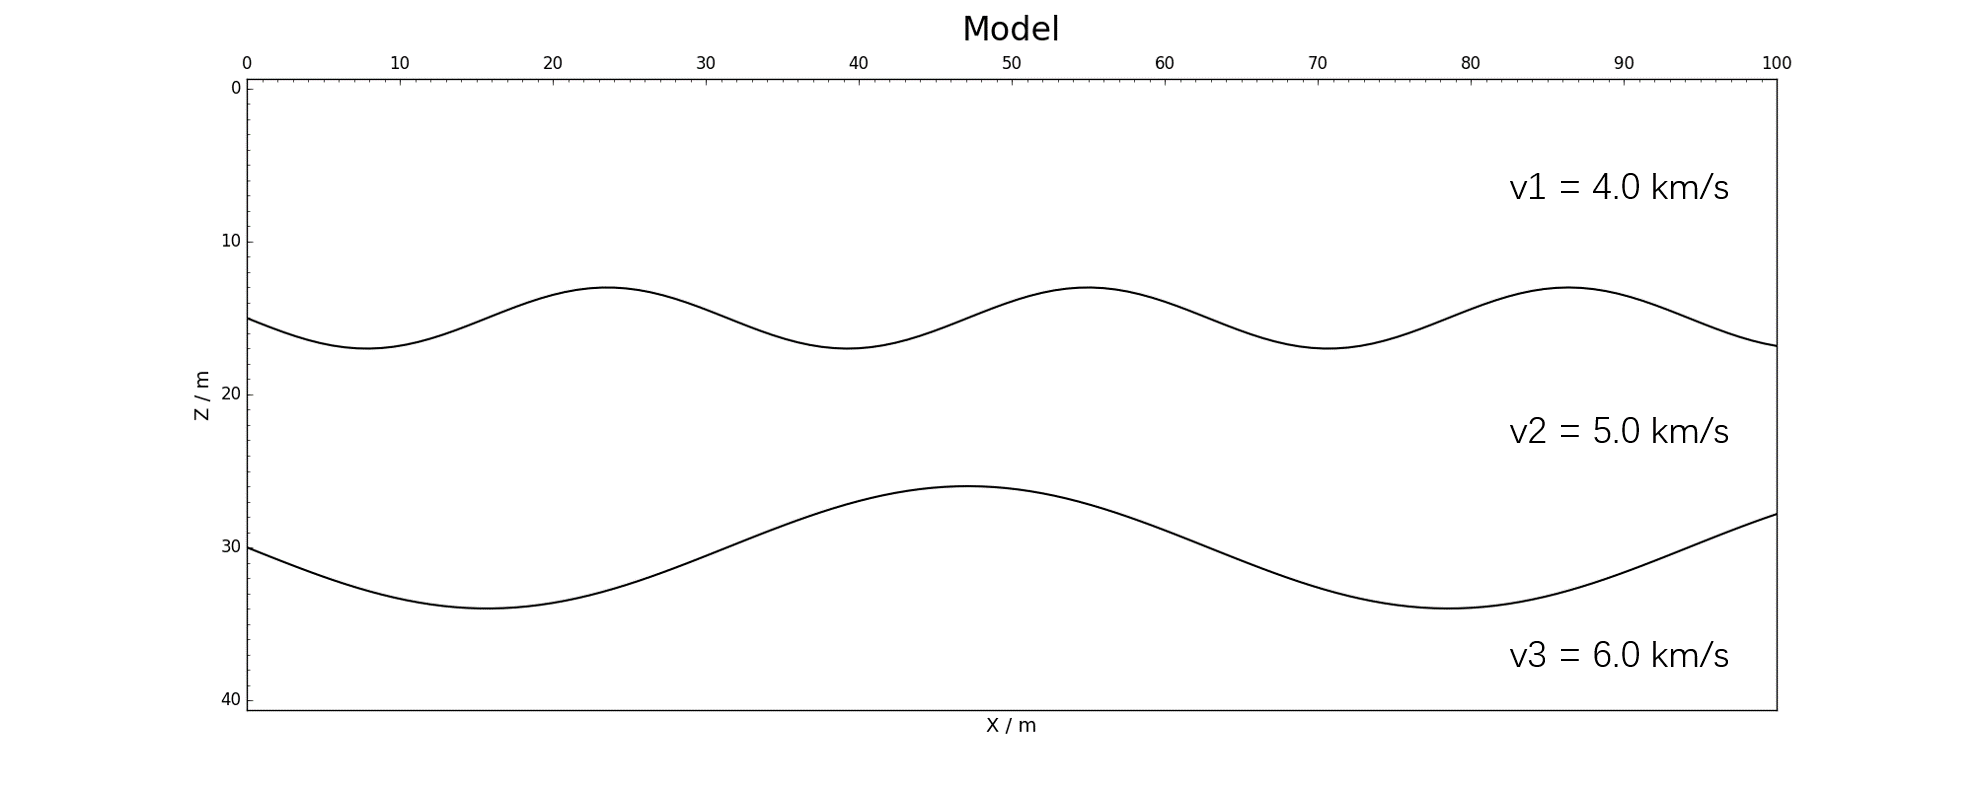
\includegraphics[scale = 0.35]{Layered_model.png}
    \end{center}
    \label{fig:Layered_model}
    \caption{Layered model}
\end{figure}

The grid we want to get from the layered model is shown in Figure \ref{fig:Grid} :
\begin{figure}[h]
    \begin{center}
        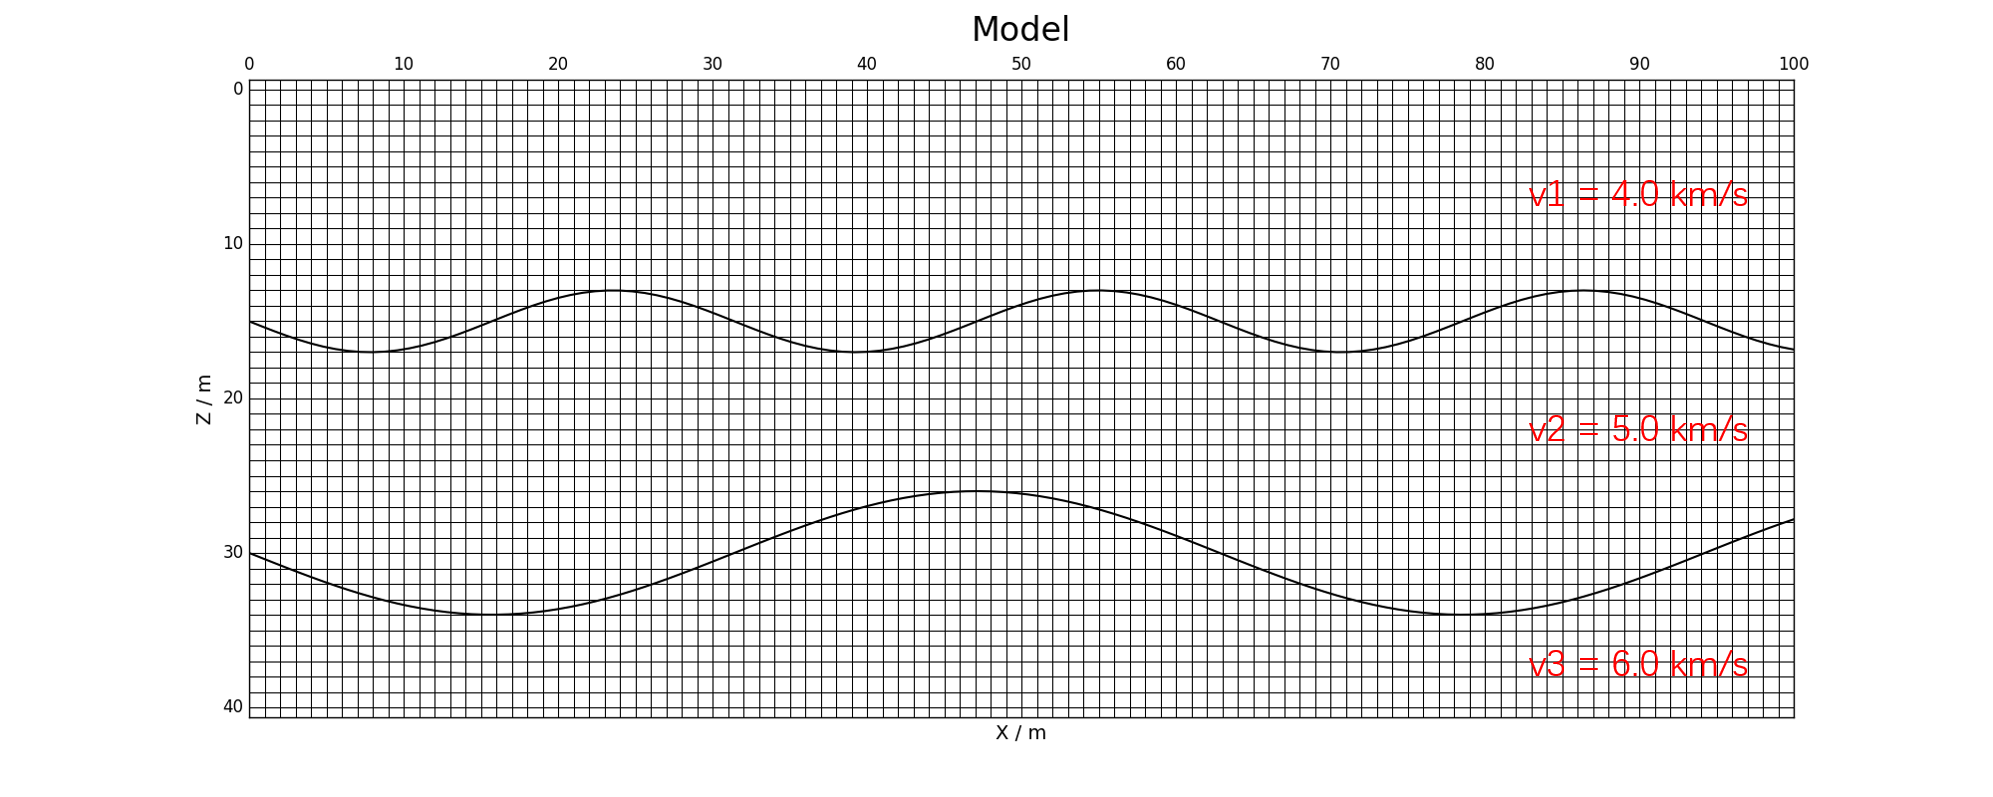
\includegraphics[scale = 0.35]{Grid.png}
    \end{center}
    \label{fig:Grid}
    \caption{Grid}
\end{figure}
